% !TEX root = ../tfg_etsiinf_NombreApellidos.tex
\chapter{Implementación} \label{chp:implementacion}

Este capítulo describe cómo se materializa en el repositorio el diseño definido
en el capítulo anterior. La atención se desplaza desde la formulación del
problema hacia la organización del software, la integración efectiva con ROS 2 y
Aerostack2, la configuración de PPO y los mecanismos de diagnóstico necesarios
para ejecutar experimentos reproducibles.

La implementación no constituye un controlador de referencia clásico. El sistema
construye una infraestructura de entrenamiento en la que Aerostack2 conserva el
control de bajo nivel, el armado, el despegue y la ejecución simulada, mientras
que la política aprendida actúa mediante comandos de velocidad compatibles con la
plataforma. Esta distinción evita atribuir a la política responsabilidades que,
en la solución desarrollada, pertenecen al \emph{stack} robótico.

\section{Organización del software} \label{sct:implementacion:organizacion}

El código desarrollado se distribuye en dos repositorios públicos. El repositorio
principal \texttt{rl\_uav\_aerostack2}\footnote{\url{https://github.com/KafeisM/rl_uav_aerostack2}}
contiene el entorno de aprendizaje, las configuraciones de entrenamiento, los
scripts de ejecución y las utilidades de validación. El repositorio
\texttt{as2\_platform\_multirotor\_simulator}\footnote{\url{https://github.com/KafeisM/as2_platform_multirotor_simulator}}
contiene el fork del simulador empleado para añadir el servicio de reinicio
determinista. Esta separación hace explícito qué parte corresponde al entorno
Gymnasium y qué parte modifica la capa física de simulación.

La implementación se organiza alrededor de tres puntos de entrada. El módulo \\
\texttt{rl\_uav/envs/as2\_test\_env.py} contiene la clase \texttt{AS2TestEnv}
y concentra la traducción entre Gymnasium y Aerostack2. El fichero
\texttt{configs/train\_ppo.yaml} define de forma declarativa los parámetros del
entorno, la vectorización, las rutas de salida y los hiperparámetros de PPO. Por
último, \texttt{scripts/train\_ppo.py} lanza el entrenamiento o valida la
configuración mediante un modo \emph{dry-run}. Esta división permite cambiar una
configuración experimental sin modificar la lógica del entorno ni los scripts de
ejecución.

El repositorio incluye además utilidades de validación para comprobar la conexión
monodron, la ejecución vectorizada, el inicio aleatorizado en hover y el
comportamiento local con \emph{mocks}. Estas comprobaciones no sustituyen a los
experimentos, pero evitan confundir errores de infraestructura con errores de
aprendizaje. En paralelo, el fork del simulador incorpora el servicio
\texttt{ResetSimulatorState}, necesario para reiniciar de forma controlada el
estado físico del multirrotor durante las campañas experimentales.

\begin{table}[H]
\centering
\footnotesize
\setlength{\tabcolsep}{4pt}
\renewcommand{\arraystretch}{1.15}

\begin{tabularx}{\textwidth}{
>{\raggedright\arraybackslash}p{0.36\textwidth}
>{\raggedright\arraybackslash}X
}
\hline
\textbf{Elemento} & \textbf{Responsabilidad principal} \\
\hline

\path{rl_uav/envs/as2_test_env.py} 
& Entorno Gymnasium y puente con Aerostack2. \\

\path{rl_uav/training/ppo_setup.py} 
& Construcción de entorno vectorizado, rutas de ejecución y modelo PPO. \\

\path{configs/train_ppo.yaml} 
& Configuración declarativa de entorno, entrenamiento e hiperparámetros. \\

\path{scripts/train_ppo.py} 
& Punto de entrada para entrenamiento y comprobación de configuración. \\

\path{scripts/as2_runtime.py} 
& Comprobación y relanzamiento controlado del simulador AS2. \\

\path{scripts/supervise_train.sh} 
& Supervisor de entrenamientos largos con reinicio del stack AS2 y reanudación desde \emph{checkpoint}. \\

\path{rl_uav/evaluation/} 
& Protocolo de evaluación por semillas con controladores enchufables, PPO y PID. \\

\path{scripts/evaluate_policy.py} 
& Punto de entrada de la evaluación formal y de la comparación entre controladores. \\

\path{as2_platform_multirotor_simulator} 
& Fork del simulador con servicio de reinicio determinista del estado del multirrotor. \\

\path{as2_sim/launch_sim.bash} 
& Arranque del simulador monodron o multidron mediante nombres de dron. \\

\path{scripts/test_*} y \path{scripts/validate_*} 
& Validaciones locales y reales del entorno, la vectorización y la integración. \\

\hline
\end{tabularx}

\caption{Organización principal del software implementado.}
\label{tab:implementacion:organizacion_software}
\end{table}

El Cuadro~\ref{tab:implementacion:organizacion_software} resume esta división.
No se busca enumerar todos los
ficheros del repositorio, sino mostrar que cada bloque tiene una responsabilidad
acotada. El entorno define la interacción, la configuración describe el
experimento, los scripts ejecutan tareas reproducibles y las utilidades de
validación reducen el riesgo de confundir un fallo de simulación con un fallo del
algoritmo.

\section{Integración con Aerostack2 y ROS 2} \label{sct:implementacion:as2_ros2}

La integración implementada toma como punto de partida la infraestructura
presentada en el Capítulo~\ref{chp:state-of-the-art}. ROS 2 aporta el grafo de
comunicación robótica y Aerostack2 proporciona la capa aérea que encapsula
operaciones como armado, modo \emph{offboard}, despegue, aterrizaje y envío de
velocidades \cite{fernandez2023aerostack2, ros2_humble_concepts}. En este
capítulo no se repite su fundamento tecnológico; se describe cómo el entorno
\texttt{AS2TestEnv} utiliza esas interfaces para convertir acciones de PPO en
órdenes ejecutables por el simulador.

La Figura~\ref{fig:implementacion:integracion_ros_as2} muestra la integración
implementada. El agente PPO interactúa únicamente con la interfaz Gymnasium. La
clase \texttt{AS2TestEnv} recibe las acciones, las convierte en comandos de
velocidad y utiliza \texttt{DroneInterface} y \texttt{SpeedMotion} para
comunicarse con Aerostack2. A su vez, Aerostack2 utiliza ROS 2 para transportar
las órdenes y estados hacia el simulador multirrotor.

\begin{figure}[t]
\centering
\shorthandoff{<>}
\begin{tikzpicture}[
    node distance=1.1cm,
    block/.style={
        rectangle,
        rounded corners,
        draw,
        align=center,
        minimum width=4.0cm,
        minimum height=0.85cm,
        font=\small
    },
    arrow/.style={-{Latex[length=2mm]}, thick}
]

\node[block] (ppo) {Política PPO\\Stable-Baselines3};
\node[block, below=of ppo] (gym) {Contrato Gymnasium\\\texttt{reset}, \texttt{step}, \texttt{close}};
\node[block, below=of gym] (env) {\texttt{AS2TestEnv}\\adaptación RL--robótica};
\node[block, below=of env] (api) {\texttt{DroneInterface} y \texttt{SpeedMotion}};
\node[block, below=of api] (ros) {ROS 2\\nodos, topics, servicios y acciones};
\node[block, below=of ros] (as2) {Aerostack2\\AS2 Multirotor Simulator};

\draw[arrow] (ppo) -- (gym);
\draw[arrow] (gym) -- (env);
\draw[arrow] (env) -- (api);
\draw[arrow] (api) -- (ros);
\draw[arrow] (ros) -- (as2);

\end{tikzpicture}
\shorthandon{<>}
\caption{Integración implementada entre la política de aprendizaje, la interfaz
Gymnasium, Aerostack2 y ROS 2.}
\label{fig:implementacion:integracion_ros_as2}
\end{figure}

En el código, la inicialización de ROS 2 se encapsula dentro de
\texttt{AS2TestEnv}. El entorno protege la llamada a \texttt{rclpy.init()} con un
bloqueo y una bandera de clase para evitar inicializaciones repetidas dentro del
mismo proceso. Esta decisión es especialmente relevante en escenarios
vectorizados, donde varias instancias lógicas del entorno pueden coexistir y
compartir recursos de ROS 2. Tras inicializar ROS 2, el entorno crea una instancia
de \texttt{DroneInterface} asociada al espacio de nombres del dron, por ejemplo
\texttt{drone0}, y una instancia de \texttt{SpeedMotion} para el envío de
velocidades.

El método \texttt{reset} ejecuta las operaciones necesarias para preparar un
episodio. Inicializa la interfaz si aún no existe, arma el dron, activa el modo
\emph{offboard}, ejecuta el despegue y genera la primera observación. El método
\texttt{step} aplica la acción emitida por el agente como
un comando de velocidad lineal y velocidad de guiñada mediante
\texttt{send\_speed\_command\_with\_yaw\_speed}. Se emplea el marco de referencia
\texttt{earth}, de forma coherente con la formulación del entorno como navegación
local hacia un objetivo relativo. El método \texttt{close}, por su parte, realiza
un cierre seguro mediante aterrizaje, paso a modo manual y liberación de la
interfaz del dron. No se apaga globalmente \texttt{rclpy} desde cada instancia,
porque hacerlo podría invalidar otras instancias activas del entorno.

El simulador se lanza desde \texttt{as2\_sim/launch\_sim.bash}. Este script
permite seleccionar el número de drones y genera nombres de espacio como
\texttt{drone0}, \texttt{drone1}, etc. Para la ejecución multidron se adopta un
criterio de un único simulador compartido con varios espacios de nombres ROS 2,
en lugar de iniciar varios simuladores independientes. Esta decisión reduce la
sobrecarga de infraestructura y se alinea con la idea de Aerostack2 como marco
capaz de operar sistemas aéreos multirrobot \cite{fernandez2023aerostack2}. Para
hacer más robusta la ejecución, \\ \texttt{scripts/as2\_runtime.py} comprueba la
existencia de las sesiones del simulador y permite relanzarlas antes de ejecutar
validaciones que dependen de AS2.

Para los experimentos con reinicio certificado se utiliza un overlay del AS2
Multirotor Simulator. El servicio añadido se expone bajo el espacio de nombres
del vehículo, por ejemplo
\texttt{/drone0/platform/reset\_simulator\_state}, y permite aplicar una pose
objetivo directamente sobre el estado del simulador. La implementación no se
limita a cambiar posición y orientación, sino que también pone a cero velocidades,
aceleraciones, fuerzas, pares y estado de motores, reinicia controlador, IMU y
odometría, y resincroniza la plataforma de Aerostack2 para dejarla armada, en
modo \emph{offboard} y en estado de vuelo.

\section{Configuración operativa de PPO} \label{sct:implementacion:ppo}

La configuración de PPO se materializa en
\texttt{configs/train\_ppo.yaml}. El Capítulo~\ref{chp:state-of-the-art}
justifica la elección del algoritmo; esta sección se limita a documentar cómo se
parametriza su uso dentro del sistema implementado y cómo se preserva la
trazabilidad de cada ejecución.

La configuración se divide en tres bloques principales. El bloque
\texttt{experiment} define el nombre del experimento, la semilla y el directorio
raíz de salida. El bloque \texttt{environment} agrupa los parámetros del entorno,
incluyendo el identificador \texttt{AS2TestEnv-v0}, el número de instancias
vectorizadas, el prefijo de espacio de nombres, los límites de posición y
velocidad, la duración de cada paso, el objetivo, las condiciones de éxito y las
penalizaciones de seguridad. El bloque \texttt{ppo} contiene los hiperparámetros
del algoritmo, como la tasa de aprendizaje, el número de pasos por actualización,
el tamaño de lote, el factor de descuento, el rango de \emph{clipping} y la
arquitectura de las redes de política y valor.

\begin{table}[H]
\centering
\small
\setlength{\tabcolsep}{4pt}
\renewcommand{\arraystretch}{1.15}
\begin{tabular}{p{0.28\textwidth} p{0.22\textwidth} p{0.40\textwidth}}
\hline
\textbf{Parámetro} & \textbf{Valor base} & \textbf{Función} \\
\hline
\texttt{total\_timesteps} & \texttt{1000000} & Duración máxima de la campaña de entrenamiento. \\
\texttt{learning\_rate} & \texttt{3.0e-05} & Tamaño de actualización de los parámetros de PPO. \\
\texttt{n\_steps} & \texttt{512} & Número de pasos recogidos antes de cada actualización. \\
\texttt{batch\_size} & \texttt{32} & Tamaño de lote usado durante la optimización. \\
\texttt{clip\_range} & \texttt{0.2} & Límite de variación entre política antigua y política nueva. \\
\texttt{use\_sde} & \texttt{true} & Activación de exploración dependiente del estado. \\
\texttt{net\_arch} & \texttt{[128, 128]} & Capas ocultas de las redes de política y valor. \\
\hline
\end{tabular}
\caption{Principales parámetros PPO definidos en la configuración base de entrenamiento.}
\label{tab:implementacion:parametros_ppo}
\end{table}

El Cuadro~\ref{tab:implementacion:parametros_ppo} recoge los parámetros más
representativos de la configuración base. Estos valores no deben interpretarse
como una optimización definitiva del algoritmo, sino como una configuración
inicial trazable y reproducible para validar la infraestructura de entrenamiento.
Los capítulos de pruebas y resultados son los que deben determinar si una
configuración concreta produce aprendizaje útil, estabilidad suficiente o
necesidad de ajuste.

A partir de Exp010 se emplea una configuración más óptima con tasa de aprendizaje \texttt{3.0e-05},
\texttt{n\_steps=512}, \texttt{batch\_size=32}, \texttt{n\_epochs=5},
\texttt{ent\_coef=0.0}, exploración SDE y redes MLP de dos capas de 128 unidades
por rama. Las configuraciones Exp010, Exp011 y Exp012 mantienen estos
hiperparámetros y modifican principalmente propiedades del entorno y de la tarea,
como la recompensa mínima, la randomización completa, los márgenes de muestreo,
el límite de distancia inicio--objetivo, los guards de acción y la reanudación de
entrenamiento. Esta separación evita mezclar ajustes del algoritmo con cambios en
las condiciones de interacción del UAV.

La configuración también explicita decisiones de ingeniería que afectan a la
reproducibilidad. El entrenamiento se fija inicialmente en CPU, coherente con el
uso de políticas MLP y con la recomendación habitual de Stable-Baselines3 para
evitar sobrecostes de GPU en redes no convolucionales. Además, se separan los
directorios de \emph{logs}, monitorización y \emph{checkpoints}, lo que permite
analizar una ejecución sin depender únicamente de la salida estándar del proceso.
Esta estructura facilita repetir experimentos, comparar configuraciones y aislar
fallos entre simulación, entorno y algoritmo.


\section{Herramientas de visualización y monitorización} \label{sct:implementacion:herramientas_monitorizacion}

La implementación se apoya en herramientas de visualización y monitorización que
permiten distinguir entre el funcionamiento del algoritmo, el estado del
simulador y la respuesta física del UAV. Esta separación es necesaria porque un
entrenamiento puede fallar por una configuración de PPO inadecuada, un reinicio
inválido del episodio, un problema de comunicación ROS 2 o una orden aceptada por
la interfaz que no produce movimiento físico.

RViz2 se utiliza como herramienta de inspección cualitativa del sistema robótico.
Aunque el simulador de multirrotores de Aerostack2 no requiere interfaz gráfica,
RViz2 permite observar la posición del UAV, la trayectoria reciente y los
marcadores publicados para representar el objetivo. Esta visualización no se usa
como métrica de aprendizaje, pero sí como apoyo para detectar comportamientos
anómalos, como ausencia de movimiento, trayectorias divergentes o incoherencias
entre el objetivo configurado y la escena simulada.

\begin{figure}[H]
\centering
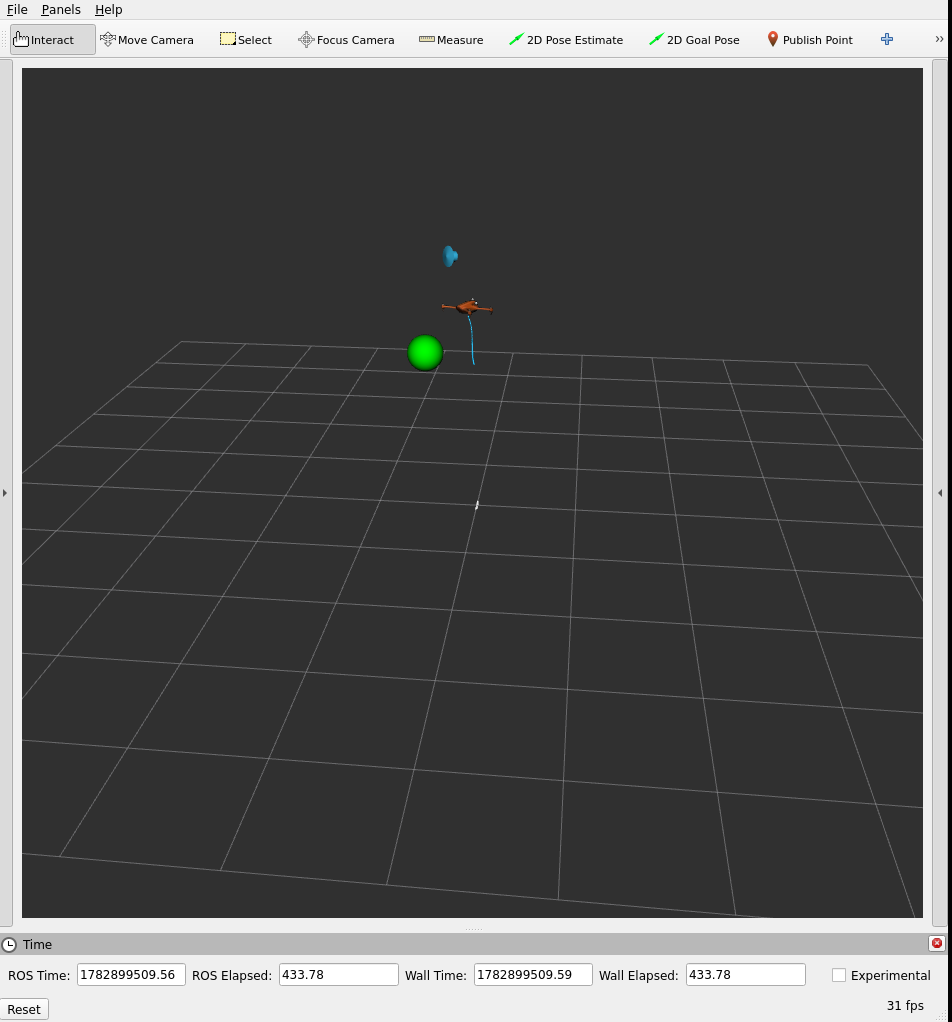
\includegraphics[width=0.82\textwidth]{images/rviz2_training_view.png}
\caption{Visualización en RViz2 del UAV simulado, la trayectoria reciente y el
marcador del objetivo durante una ejecución con Aerostack2.}
\label{fig:implementacion:rviz2_training_view}
\end{figure}

La Figura~\ref{fig:implementacion:rviz2_training_view} muestra un ejemplo de la
visualización empleada durante las pruebas. El marcador verde representa el
objetivo de navegación y el modelo del UAV permite comprobar de forma cualitativa
si el movimiento observado es coherente con las acciones enviadas por el entorno.

TensorBoard se emplea como herramienta de monitorización de las métricas emitidas
por Stable-Baselines3 y por los monitores vectorizados. En las ejecuciones en las
que PPO alcanza suficientes pasos para completar una primera actualización, esta
herramienta permite inspeccionar magnitudes como recompensa media por episodio,
longitud media de episodio y otros escalares registrados. Sin embargo, la
interpretación de TensorBoard debe realizarse junto con los ficheros de monitor y
los diagnósticos del entorno. Una curva ausente o congelada puede indicar que el
entrenamiento no ha alcanzado un \emph{rollout} completo, que el proceso se ha
bloqueado durante un reset o que el simulador ha dejado de producir transiciones
válidas.

\begin{table}[H]
\centering
\small
\setlength{\tabcolsep}{4pt}
\renewcommand{\arraystretch}{1.15}
\begin{tabular}{p{0.25\textwidth} p{0.62\textwidth}}
\hline
\textbf{Herramienta} & \textbf{Uso en el trabajo} \\
\hline
ROS 2 & Comunicación entre nodos, servicios, acciones y flujos de datos del sistema robótico. \\
Aerostack2 & Capa aérea reutilizada para armado, modos de vuelo, control y simulación. \\
AS2 Multirotor Simulator & Simulación dinámica del multirrotor usado como fuente de experiencia. \\
Gymnasium & Interfaz estándar del entorno de aprendizaje por refuerzo. \\
Stable-Baselines3 & Implementación de PPO y utilidades de entrenamiento. \\
TensorBoard & Monitorización de escalares y evolución de métricas durante ejecuciones PPO. \\
RViz2 & Visualización cualitativa del UAV, el objetivo y la trayectoria en el espacio simulado. \\
\hline
\end{tabular}
\caption{Herramientas principales utilizadas durante la implementación y validación.}
\label{tab:implementacion:herramientas}
\end{table}


\section{Implementación del entorno de aprendizaje} \label{sct:implementacion:entorno}

La clase \texttt{AS2TestEnv} materializa el diseño del
Capítulo~\ref{chp:diseno}. En lugar de volver a justificar los espacios de
observación y acción, esta sección se centra en cómo se ejecuta el contrato en el
código. El entorno registra \texttt{AS2TestEnv-v0}, define los espacios
\texttt{Box} correspondientes, aplica los límites configurados y encapsula las
operaciones de ciclo de vida que requiere Aerostack2.

Durante \texttt{reset}, el entorno prepara la interfaz robótica, arma el UAV,
activa el modo \emph{offboard}, ejecuta el despegue y devuelve la primera
observación normalizada. Cuando se habilita \texttt{randomize\_hover\_start}, la
posición inicial, la guiñada y el objetivo se muestrean dentro de los límites
configurados. Exp011 añade márgenes en XY y altura, junto con
\texttt{max\_start\_target\_distance}, para evitar episodios que comiencen junto
a fronteras problemáticas o con la observación saturada desde el primer paso.

Durante \texttt{step}, la acción recibida se recorta mediante \texttt{max\_vel} y
\texttt{max\_yaw\_vel}, se envía a Aerostack2 con \texttt{SpeedMotion} y se lee el
estado actualizado del UAV. Con esa información se calcula la recompensa, se
evalúan las condiciones de terminación y se generan campos de diagnóstico.

\begin{figure}[t]
\centering
\shorthandoff{<>}
\begin{tikzpicture}[
    node distance=1.05cm and 1.5cm,
    block/.style={
        rectangle,
        rounded corners,
        draw,
        align=center,
        minimum width=3.1cm,
        minimum height=0.8cm,
        font=\small
    },
    arrow/.style={-{Latex[length=2mm]}, thick}
]

\node[block] (reset) {\texttt{reset()}\\preparación del episodio};
\node[block, below=of reset] (obs0) {Observación inicial};
\node[block, below=of obs0] (policy) {Política PPO\\selección de acción};
\node[block, below=of policy] (action) {Acción limitada\\velocidad y yaw};
\node[block, below=of action] (step) {\texttt{step()}\\envío a AS2};
\node[block, below left=of step] (reward) {Recompensa\\distancia + terminales};
\node[block, below right=of step] (end) {Terminación o\\truncamiento};

\draw[arrow] (reset) -- (obs0);
\draw[arrow] (obs0) -- (policy);
\draw[arrow] (policy) -- (action);
\draw[arrow] (action) -- (step);
\draw[arrow] (step) -- (reward);
\draw[arrow] (step) -- (end);
\draw[arrow] (reward.west) .. controls +(-2.0,0) and +(-2.0,0) .. (policy.west);

\end{tikzpicture}
\shorthandon{<>}
\caption{Ciclo implementado de un episodio de aprendizaje por refuerzo sobre
\texttt{AS2TestEnv}.}
\label{fig:implementacion:ciclo_entorno}
\end{figure}

La Figura~\ref{fig:implementacion:ciclo_entorno} resume el flujo implementado.
La responsabilidad principal del entorno no es definir de nuevo el problema de
aprendizaje, sino convertir cada interacción de PPO en una operación robótica
acotada, observable y registrable.


\section{Diagnóstico del reinicio y de la accionabilidad} \label{sct:implementacion:diagnostico_reset}

La implementación añade un paso específico porque el entrenamiento solo
es válido si el UAV parte de un estado físico coherente y responde a las acciones
enviadas. Por este motivo, el entorno registra el método de reinicio, el camino
seguido, el estado del servicio, los errores residuales de posición y guiñada, el
desplazamiento físico, la longitud de trayectoria, la aceptación de comandos y la
altitud mínima. Estos campos permiten distinguir un fallo de aprendizaje de un
fallo previo de simulación o de accionabilidad.

El parámetro \texttt{reset\_max\_vel} separa la autoridad usada por los comandos
internos de reinicio de la velocidad máxima permitida a PPO. Por otra parte cabe
destacar que cuando la interfaz, acepta comandos pero el UAV no se desplaza de forma apreciable, 
el entorno falla
de forma cerrada y evita generar experiencia inválida.

El servicio \texttt{ResetSimulatorState}, añadido en el fork del simulador,
aplica una pose objetivo y reinicia velocidades, aceleraciones, fuerzas, pares,
motores, controlador, IMU y odometría. Sobre ese servicio se implementan
reintentos mediante \\ \texttt{reset\_service\_max\_attempts} y
\texttt{reset\_service\_retry\_backoff\_s}. Exp010 mostró que abortar tras un
fallo transitorio era demasiado frágil; Exp011 añadió reintentos, y Exp012 redujo
la frecuencia de reinicios forzados mediante un guard de acción en fronteras.

El guard de Exp012 modifica las acciones que empujan al UAV hacia fuera cuando se
aproxima a los límites XY o al techo de la escena. Las terminaciones por salida
de límites y baja altitud se mantienen como red de seguridad, pero dejan de ser
el mecanismo habitual para corregir a un agente aún no entrenado. A partir de
Exp013 el disparo de ambos guards es predictivo: se evalúa la posición estimada
como posición actual más velocidad medida por un horizonte configurable
(\texttt{bounds\_guard\_lookahead\_s},
\texttt{low\_altitude\_guard\_lookahead\_s}), y el empuje vertical dispone de
autoridad completa (\texttt{bounds\_guard\_vertical\_push\_speed}), porque los
datos de Exp012 mostraron que la inercia vertical atravesaba un guard puramente
reactivo (404 de 428 salidas de límites se produjeron por techo o suelo).

Para la ejecución vectorizada se implementa además el mecanismo de vigilancia de
comandos inactivos descrito en el diseño. Un hilo de fondo comprueba el tiempo
transcurrido desde la última referencia de movimiento enviada por cualquier vía
(pasos del agente, comandos de reinicio o sondas de accionabilidad); si el
vehículo está en vuelo y ese tiempo supera \texttt{idle\_command\_watchdog\_s},
publica referencias de velocidad nula a la cadencia de publicación configurada
hasta que el flujo normal se reanuda. La validación en vivo del mecanismo redujo
la deriva por referencias persistentes de 8,05 m a 0,27 m en una ventana de 20 s
sin comandos. El parámetro vale cero por defecto, de modo que la ejecución
monodron no crea el hilo ni altera su comportamiento.


\section{Infraestructura de entrenamiento y vectorización} \label{sct:implementacion:infraestructura_entrenamiento}

La infraestructura de entrenamiento se concentra en \texttt{ppo\_setup.py}. Este
módulo carga la configuración, crea los directorios de salida, instancia los
entornos, envuelve la ejecución con \texttt{VecMonitor} y construye el modelo PPO.
El registro de métricas se realiza sobre el entorno vectorizado para obtener
estadísticas de episodio agregadas sin duplicar lógica de monitorización en cada
instancia.

La vectorización se implementa mediante espacios de nombres ROS 2. A partir del
prefijo \texttt{drone} se generan instancias como \texttt{drone0},
\texttt{drone1}, \texttt{drone2}, ... , \texttt{droneN}, todas conectadas al mismo
simulador compartido. Esta solución evita lanzar un simulador por entorno y
mantiene la correspondencia entre instancia de Gymnasium y UAV simulado. La
implementación puede usar \texttt{DummyVecEnv} o \texttt{SubprocVecEnv} según la
configuración, aunque la validación inicial prioriza ejecuciones controladas
antes que paralelización agresiva.

El entrenamiento se ejecuta en dos pasos explícitos. Primero se lanza o verifica
el simulador con los scripts de AS2; después se ejecuta
\texttt{scripts/train\_ppo.py} con la configuración seleccionada. Para campañas
largas, \texttt{train\_ppo.py} acepta \texttt{--resume-from}, que reanuda desde
un \emph{checkpoint} explícito o desde el más reciente y calcula el número de
pasos restante hasta el total configurado (Stable-Baselines3 suma el argumento al
contador del \emph{checkpoint}, por lo que pasar el total completo duplicaría el
objetivo en cada reanudación).

El supervisor \texttt{scripts/supervise\_train.sh} automatiza tres mecanismos
sobre esa base. Ante un fallo del entrenamiento, reinicia el stack AS2 completo,
espera a que el servicio de reinicio de cada dron esté disponible y reanuda desde
el último \emph{checkpoint}. Mediante la variable \texttt{RECYCLE\_SECONDS}
aplica además un reciclado preventivo donde interrumpe el entrenamiento a intervalos
fijos y lo reanuda sobre un stack recién iniciado, de modo que cada tramo se
ejecuta sobre un simulador sin degradación acumulada; los reciclados se detectan
por el tiempo transcurrido, no solo por el código de salida, y no consumen el
presupuesto de reintentos por fallo. Por último, \texttt{DRONE\_NAMESPACES}
extiende el reinicio y la comprobación de salud a varios drones para las campañas
vectorizadas, e \texttt{INITIAL\_RESUME} permite sembrar una etapa del curriculum
con el modelo final de la etapa anterior cuando aún no existen \emph{checkpoints}
propios.

La validación inicial confirma que el pipeline puede crear el modelo PPO,
conectarse con AS2, enviar comandos de velocidad y generar trazas
monitorizables. Esta evidencia prueba la infraestructura de entrenamiento, no el
rendimiento final de la política; esa interpretación corresponde a los capítulos
de pruebas y resultados.
